La macchina a stati modellata, a livello concettuale, può essere divisa in due sezioni principali: la sezione di lettura (gestita dagli stati compresi tra S\textsubscript{0} e S\textsubscript{8}) e la sezione di scrittura( gestita dagli stati compresi tra S\textsubscript{9} e S\textsubscript{14}).

S\textsubscript{0} è lo stato di Reset della macchina e quest'ultima rimane in questo stato fino a quando non riceve il segnale 'i\_start' alto, che indica che può iniziare la conversione dell'immagine.

Gli stati S\textsubscript{1}, S\textsubscript{2}, S\textsubscript{3}, S\textsubscript{4}, S\textsubscript{5} si occupano di inizializzare correttamente i vari registri dei moduli precedentemente illustrati, tra cui: c\_max register, r\_max register, max register e min register.
In caso di dimensioni nulle dell'immagine (segnalate dal row\_counter module o dal column\_counter module rispettivamente tramite i segnali row\_zero e column\_zero), la macchina si sposta nello stato S\textsubscript{14} che viene descritto più nel dettaglio in seguito, altrimenti si sposta nello stato S\textsubscript{6}.

Gli stati S\textsubscript{6}, S\textsubscript{7}, S\textsubscript{8} si occupano di effettuare la lettura corretta dell'immagine e di individuare i valori di massima e minima intensità assunti dai pixel. Più precisamente, gli stati S\textsubscript{6} e S\textsubscript{8} gestiscono il nested loop descritto nella sezione \textbf{Row \& Column counter}, infatti i segnali c\_done e r\_done, una volta posti a '1', segnalano rispettivamente la fine di una riga e la fine dell'immagine.


\begin{center}
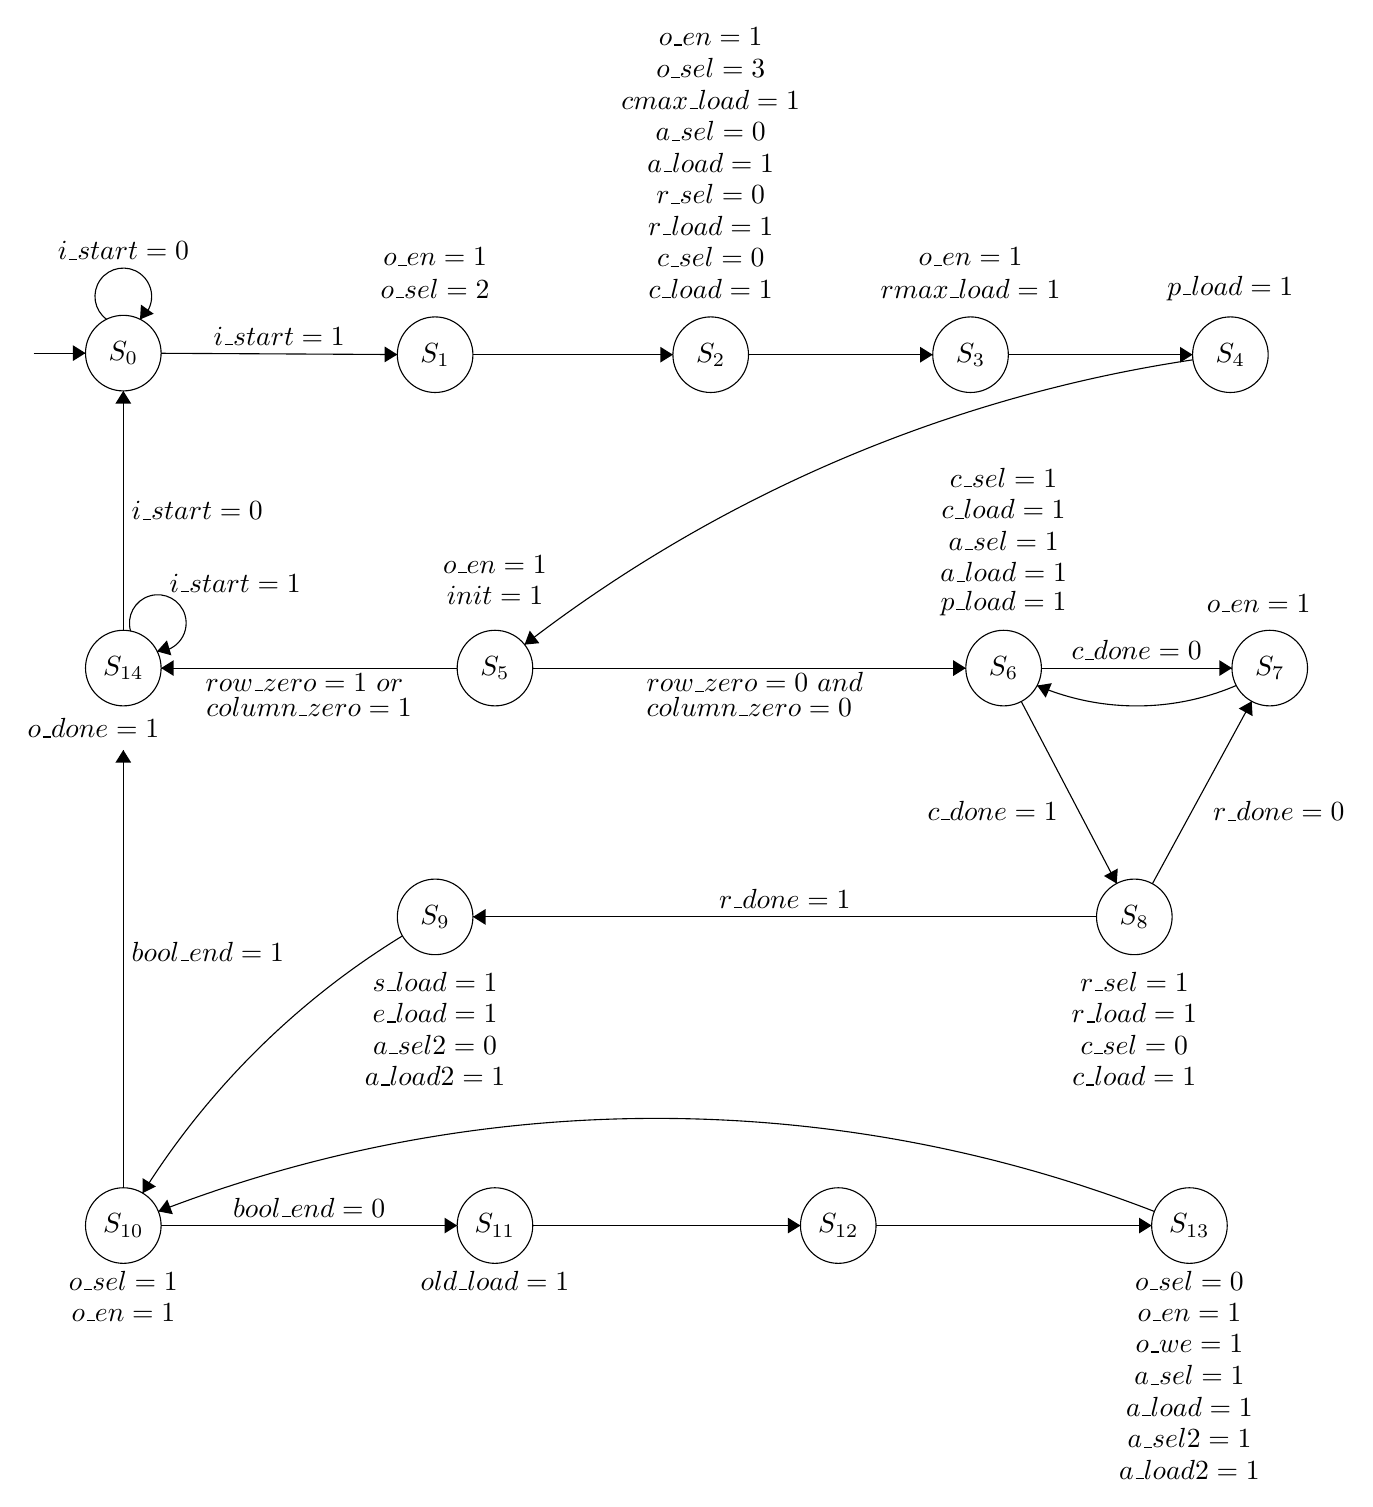
\begin{tikzpicture}[scale=0.2]
\tikzstyle{every node}+=[inner sep=0pt]
\draw [black] (5.9,-5.6) circle (2.4);
\draw (5.9,-5.6) node {$S_0$};
\draw [black] (25.7,-5.7) circle (2.4);
\draw (25.7,-5.7) node {$S_1$};
\draw [black] (43.2,-5.7) circle (2.4);
\draw (43.2,-5.7) node {$S_2$};
\draw [black] (59.7,-5.7) circle (2.4);
\draw (59.7,-5.7) node {$S_3$};
%S1
\draw (25.7,+0.5) node {$o\_en=1$};
\draw (25.7,-1.5) node {$o\_sel=2$};
%S2
\draw (43.2,+14.5) node {$o\_en=1$};
\draw (43.2,+12.5) node {$o\_sel=3$};
\draw (43.2,+10.5) node {$cmax\_load=1$};
\draw (43.2,+8.5) node {$a\_sel=0$};
\draw (43.2,+6.5) node {$a\_load=1$};
\draw (43.2,+4.5) node {$r\_sel=0$};
\draw (43.2,+2.5) node {$r\_load=1$};
\draw (43.2,+0.5) node {$c\_sel=0$};
\draw (43.2,-1.5) node {$c\_load=1$};
%S3
\draw (59.7,+0.5) node {$o\_en=1$};
\draw (59.7,-1.5) node {$rmax\_load=1$};
%S4
\draw (76.2,-1.5) node {$p\_load=1$};
%S5
\draw (29.5,-21) node {$init=1$};
\draw (29.5,-19) node {$o\_en=1$};
%S6
\draw (61.8,-13.5) node {$c\_sel=1$};
\draw (61.8,-15.5) node {$c\_load=1$};
\draw (61.8,-17.5) node {$a\_sel=1$};
\draw (61.8,-19.5) node {$a\_load=1$};
\draw (61.8,-21.5) node {$p\_load=1$};
%S7
\draw (78,-21.5) node {$o\_en=1$};
%S8
\draw (70.1,-45.5) node {$r\_sel=1$};
\draw (70.1,-47.5) node {$r\_load=1$};
\draw (70.1,-49.5) node {$c\_sel=0$};
\draw (70.1,-51.5) node {$c\_load=1$};
%S9
\draw (25.7,-45.5) node {$s\_load=1$};
\draw (25.7,-47.5) node {$e\_load=1$};
\draw (25.7,-49.5) node {$a\_sel2=0$};
\draw (25.7,-51.5) node {$a\_load2=1$};
%S10
\draw (5.9,-64.5) node {$o\_sel=1$};
\draw (5.9,-66.5) node {$o\_en=1$};
%S11
\draw (29.5,-64.5) node {$old\_load=1$};
%S12

%S13
\draw (73.6,-64.5) node {$o\_sel=0$};
\draw (73.6,-66.5) node {$o\_en=1$};
\draw (73.6,-68.5) node {$o\_we=1$};
\draw (73.6,-70.5) node {$a\_sel=1$};
\draw (73.6,-72.5) node {$a\_load=1$};
\draw (73.6,-74.5) node {$a\_sel2=1$};
\draw (73.6,-76.5) node {$a\_load2=1$};
%S14
\draw (4,-29.4) node {$o\_done=1$};

\draw [black] (76.2,-5.7) circle (2.4);
\draw (76.2,-5.7) node {$S_4$};
\draw [black] (29.5,-25.6) circle (2.4);
\draw (29.5,-25.6) node {$S_5$};
\draw [black] (61.8,-25.6) circle (2.4);
\draw (61.8,-25.6) node {$S_6$};
\draw [black] (78.7,-25.6) circle (2.4);
\draw (78.7,-25.6) node {$S_7$};
\draw [black] (70.1,-41.4) circle (2.4);
\draw (70.1,-41.4) node {$S_8$};
\draw [black] (25.7,-41.4) circle (2.4);
\draw (25.7,-41.4) node {$S_9$};
\draw [black] (5.9,-61) circle (2.4);
\draw (5.9,-61) node {$S_{10}$};
\draw [black] (29.5,-61) circle (2.4);
\draw (29.5,-61) node {$S_{11}$};
\draw [black] (51.3,-61) circle (2.4);
\draw (51.3,-61) node {$S_{12}$};
\draw [black] (73.6,-61) circle (2.4);
\draw (73.6,-61) node {$S_{13}$};
\draw [black] (5.9,-25.6) circle (2.4);
\draw (5.9,-25.6) node {$S_{14}$};
\draw (17.4,-26.5) node {$row\_zero=1\mbox{ }or$};
\draw (46,-26.5) node {$row\_zero=0\mbox{ }and$};
\draw [black] (8.3,-5.61) -- (23.3,-5.69);
\fill [black] (23.3,-5.69) -- (22.5,-5.18) -- (22.5,-6.18);
\draw (15.8,-5.13) node [above] {$i\_start=1$};
\draw [black] (0.2,-5.6) -- (3.5,-5.6);
\fill [black] (3.5,-5.6) -- (2.7,-5.1) -- (2.7,-6.1);
\draw [black] (4.842,-3.456) arc (234:-54:1.8);
\draw (5.9,0.3) node [above] {$i\_start=0$};
\fill [black] (6.96,-3.46) -- (7.83,-3.1) -- (7.02,-2.52);
\draw [black] (28.1,-5.7) -- (40.8,-5.7);
\fill [black] (40.8,-5.7) -- (40,-5.2) -- (40,-6.2);
\draw [black] (45.6,-5.7) -- (57.3,-5.7);
\fill [black] (57.3,-5.7) -- (56.5,-5.2) -- (56.5,-6.2);
\draw [black] (62.1,-5.7) -- (73.8,-5.7);
\fill [black] (73.8,-5.7) -- (73,-5.2) -- (73,-6.2);
\draw [black] (31.381,-24.109) arc (127.6527:98.50736:91.678);
\fill [black] (31.38,-24.11) -- (32.32,-24.02) -- (31.71,-23.22);
\draw [black] (31.9,-25.6) -- (59.4,-25.6);
\fill [black] (59.4,-25.6) -- (58.6,-25.1) -- (58.6,-26.1);
\draw (45.65,-28.7) node [above] {$column\_zero=0$};
\draw [black] (27.1,-25.6) -- (8.3,-25.6);
\fill [black] (8.3,-25.6) -- (9.1,-26.1) -- (9.1,-25.1);
\draw (17.7,-28.7) node [above] {$column\_zero=1$};
\draw [black] (64.2,-25.6) -- (76.3,-25.6);
\fill [black] (76.3,-25.6) -- (75.5,-25.1) -- (75.5,-26.1);
\draw (70.25,-25.1) node [above] {$c\_done=0$};
\draw [black] (76.573,-26.706) arc (-66.80792:-113.19208:16.055);
\fill [black] (63.93,-26.71) -- (64.47,-27.48) -- (64.86,-26.56);
\draw [black] (62.92,-27.72) -- (68.98,-39.28);
\fill [black] (68.98,-39.28) -- (69.05,-38.33) -- (68.17,-38.8);
\draw (65.27,-34.65) node [left] {$c\_done=1$};
\draw [black] (71.25,-39.29) -- (77.55,-27.71);
\fill [black] (77.55,-27.71) -- (76.73,-28.17) -- (77.61,-28.65);
\draw (75.07,-34.68) node [right] {$r\_done=0$};
\draw [black] (67.7,-41.4) -- (28.1,-41.4);
\fill [black] (28.1,-41.4) -- (28.9,-41.9) -- (28.9,-40.9);
\draw (47.9,-40.9) node [above] {$r\_done=1$};
\draw [black] (7.126,-58.937) arc (147.92027:121.49805:50.79);
\fill [black] (7.13,-58.94) -- (7.97,-58.52) -- (7.13,-57.99);
\draw [black] (8.3,-61) -- (27.1,-61);
\fill [black] (27.1,-61) -- (26.3,-60.5) -- (26.3,-61.5);
\draw (17.7,-60.5) node [above] {$bool\_end=0$};
\draw [black] (31.9,-61) -- (48.9,-61);
\fill [black] (48.9,-61) -- (48.1,-60.5) -- (48.1,-61.5);
\draw [black] (53.7,-61) -- (71.2,-61);
\fill [black] (71.2,-61) -- (70.4,-60.5) -- (70.4,-61.5);
\draw [black] (8.126,-60.103) arc (111.17339:68.82661:87.555);
\fill [black] (8.13,-60.1) -- (9.05,-60.28) -- (8.69,-59.35);
\draw [black] (5.9,-23.2) -- (5.9,-8);
\fill [black] (5.9,-8) -- (5.4,-8.8) -- (6.4,-8.8);
\draw [black] (5.9,-58.6) -- (5.9,-30.8);
\fill [black] (5.9,-30.8) -- (5.4,-31.6) -- (6.4,-31.6);
\draw (6.4,-43.6) node [right] {$bool\_end=1$};
\draw [black] (6.365,-23.255) arc (196.51907:-91.48093:1.8);
\draw (13,-20.82) node [above] {$i\_start=1$};
\fill [black] (8.04,-24.54) -- (8.95,-24.79) -- (8.67,-23.84);
\draw (6.4,-15.6) node [right] {$i\_start=0$};
\end{tikzpicture}
\end{center}

%\end{document}
